\section{Intrinsic Parameters}

\begin{figure}[h!]
    \centering
    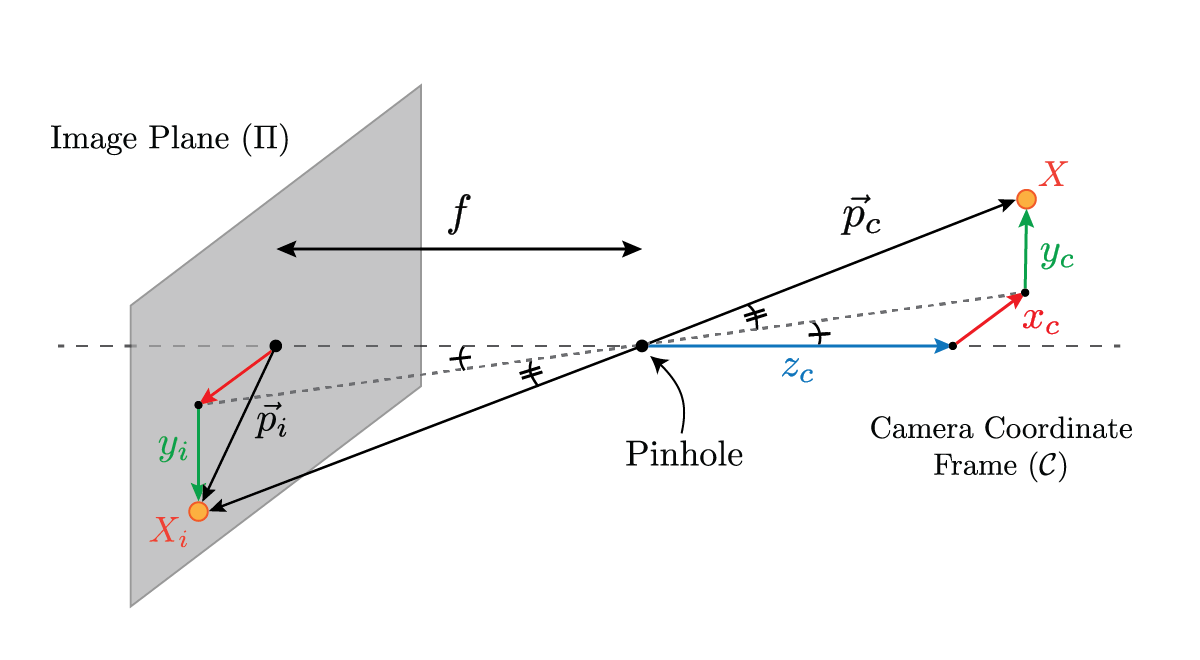
\includegraphics[width=0.9\textwidth]{figures/perspective_projection}
    \caption{Perspective projection.}
\end{figure}

\begin{figure}[h!]
    \centering
    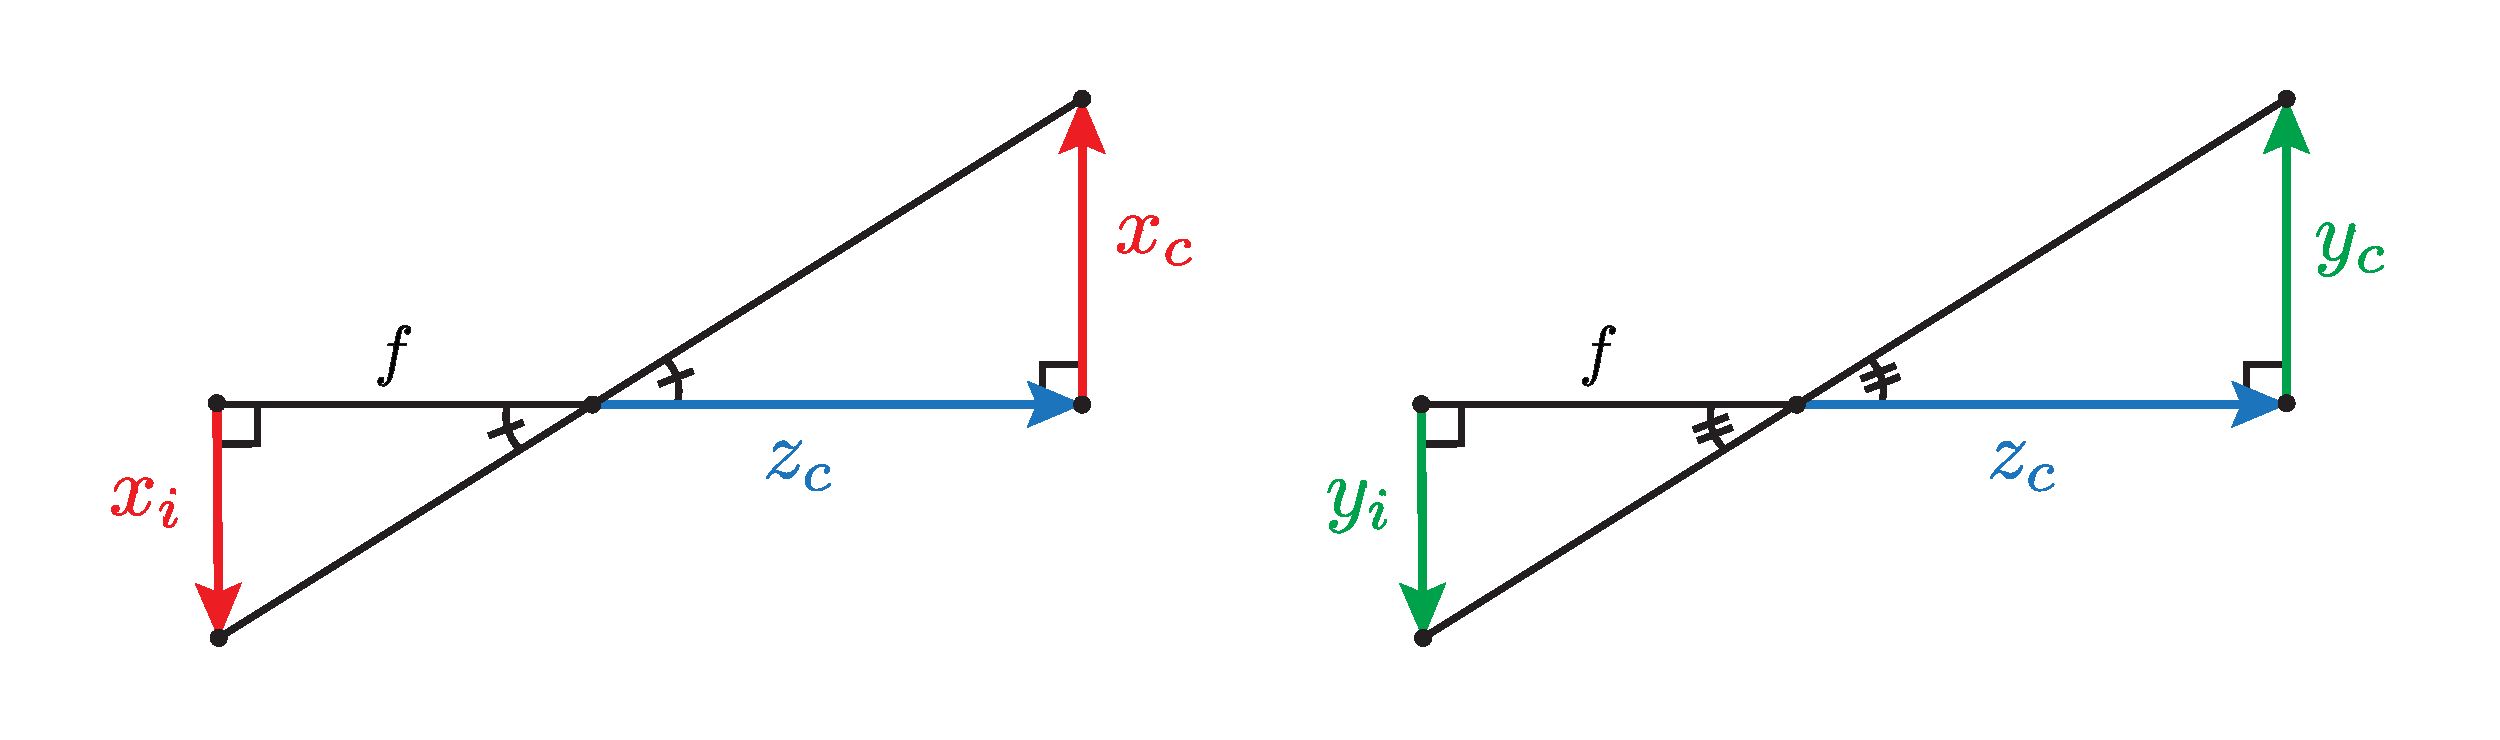
\includegraphics[width=\textwidth]{figures/similar_triangles}
    \caption{Similar triangles formed by perspective projection.}
\end{figure}

\begin{gather}
    \frac{x_i}{f} = \frac{x_c}{z_c} \Rightarrow x_i = f \frac{x_c}{z_c} \\
    \frac{y_i}{f} = \frac{y_c}{z_c} \Rightarrow y_i = f \frac{y_c}{z_c}
\end{gather}

\begin{figure}[h!]
    \centering
    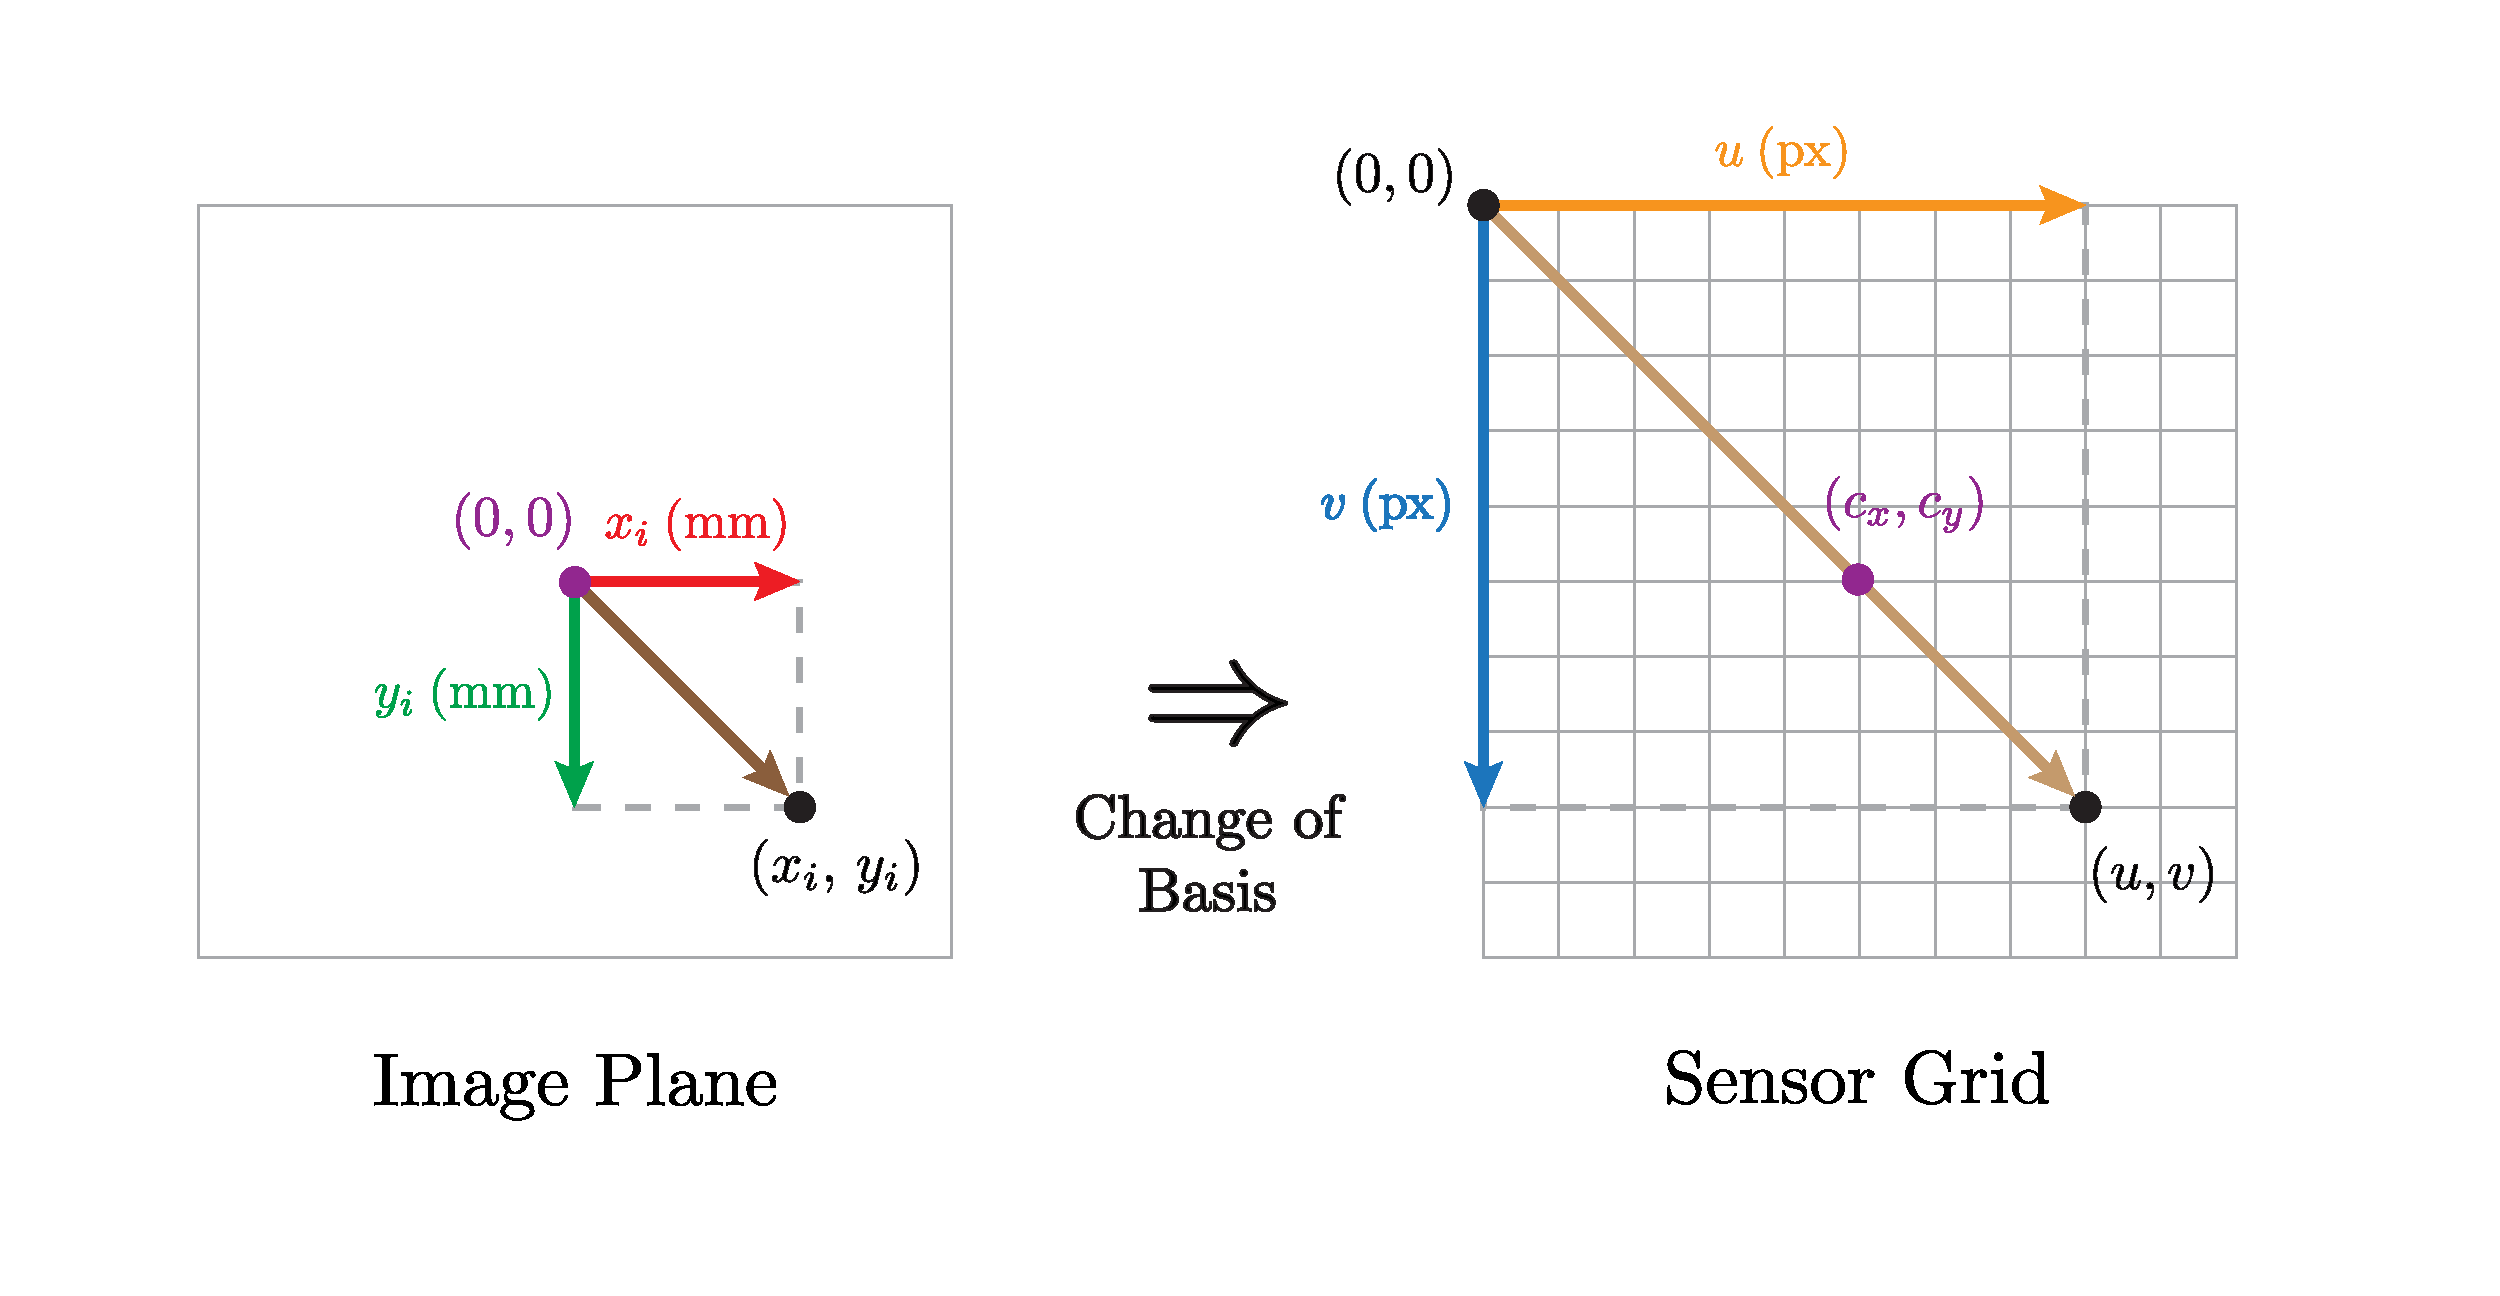
\includegraphics[width=\textwidth]{figures/sensor_grid}
    \caption{Conversion from image plane coordinates to sensor grid coordinates}
\end{figure}


Let $m_x$ and $m_y$ represent the pixel density of the image sensor in the $x$ and $y$ axes of the image sensor plane respectively.


\begin{align*}
    u = m_x x_i + c_x \\
    v = m_y y_i + c_y
\end{align*}

\begin{align*}
    u = m_x f \frac{x_c}{z_c} + c_x \\
    v = m_y f \frac{y_c}{z_c} + c_y
\end{align*}

\begin{subequations}
    \begin{gather}
        u = f_x \frac{x_c}{z_c} + c_x \\
        v = f_y \frac{y_c}{z_c} + c_y
    \end{gather}
\end{subequations}

We can linearize 

\begin{equation}
    \begin{bmatrix}
        u \\ v \\ 1
    \end{bmatrix}
    \equiv
    \begin{bmatrix}
        \widetilde{u} \\ \widetilde{v} \\ \widetilde{w}
    \end{bmatrix}
    \equiv
    \begin{bmatrix}
        z_c u \\ z_c v \\ z_c
    \end{bmatrix}
    =
    \begin{bmatrix}
        f_x x_c + z_c c_x \\ f_y y_c + z_c c_y \\ z_c
    \end{bmatrix} 
    =
    \underbrace{
    \begin{bmatrix}
        f_x & 0   & c_x & 0 \\
        0   & f_y & c_y & 0 \\
        0   & 0   & 1   & 0
    \end{bmatrix}
    }_{M_{int}}
    \begin{bmatrix}
        x_c \\ y_c \\ z_c \\ 1
    \end{bmatrix}
\end{equation}
